\documentclass[a4paper,12pt]{article}

% Sets margins
\usepackage[margin=1in]{geometry}

% To draw the skill circles
\usepackage{tikz}
\usetikzlibrary{calc,fadings,shadings}

\tikzfading[name=fade out,inner color=transparent!0,outer color=transparent!100]
\newcommand{\skilldisk}[1]{%
 \def\sbcolor{red}
 \hspace{.5em}%
 \def\R{.15cm}%
 \begin{tikzpicture}[remember picture]%
  \pgfmathsetmacro\A{90-3.6*#1}
  \def\bgcolor{gray!40}
  \def\fgcolor{\sbcolor!50}
  
  \fill [white] (0,0) circle (\R);
  
  \shade[ball color = \bgcolor, opacity = 0.4] (0,0) circle (\R);
  \shade[ball color = \fgcolor, opacity = 0.8] (0,\R) arc (90:\A:\R) -- (0,0) -- cycle;
 \end{tikzpicture}%
}

% For hyperlinks, as usual
\usepackage{hyperref}

% Main tabular layout
% \usepackage{booktabs} % Surprisingly un-used here
\usepackage{longtable} % Pagebreak-able tables
\usepackage{makecell} % Encapsulated tabular cell contents

% The list of publications (with links)
\usepackage[backend=biber,maxcitenames=1,doi=false,isbn=false,url=false,sorting=ydnt]{biblatex}
\addbibresource{cv.bib}

% The euro symbol
\usepackage{eurosym}

% Symbols in the contact section
\usepackage{fontawesome}

 % To compute available rspace based on lspace
\usepackage{calc}

% Put pages number in footer
\usepackage{lastpage}
\usepackage{fancyhdr}

\def\fancysize{\small}

\fancyfoot[C]{\fancysize \thepage\ of \pageref*{LastPage}}
\fancyhead{}
 
\fancypagestyle{fancyfirst}{
 \fancyhead{}
 \fancyfoot[L]{\fancysize Updated on \today{}}
 \fancyfoot[C]{\fancysize \faRefresh \href{https://github.com/kgd-al/CV/raw/master/cv.pdf}{Up-to date version}}
 \fancyfoot[R]{\fancysize \footnotesize Page \thepage\ of \pageref*{LastPage}}
}

\renewcommand{\headrulewidth}{0pt}
\pagestyle{fancy}
\thispagestyle{fancyfirst}

% For (excessively) pretty underlining
\usepackage{contour}
\usepackage[normalem]{ulem}
\renewcommand{\ULdepth}{2pt}
\contourlength{0.8pt}
\newcommand{\prettyuline}[1]{%
 \uline{\phantom{#1}}%
 \llap{\contour{white}{#1}}%
}

% Helper for the mail links
\def\mailto#1{\small\href{mailto:#1}{\texttt{#1}}}

% Pdf meta-data
\def\me{Kevin Godin-Dubois}
\makeatletter
\hypersetup{
 pdfinfo={
  Author={\me},
  Title={\me{} - CV}
 }
}
\makeatother

% No indent
\setlength\parindent{0pt}

% =============================================================================
% Draft section

% To monitor file inclusion (in git)
\listfiles 

% Overfull hbox debugging
\overfullrule=1mm

% =============================================================================
\begin{document}

% Prepare lengths
\newlength\lwidth
\setlength\lwidth{.2\textwidth}
\newlength\cwidth
\setlength\cwidth{\dimexpr2\tabcolsep}
\newlength\rwidth
\setlength\rwidth{\dimexpr\textwidth-\lwidth-\cwidth-.4pt}

% Local variables
\newlength\titlewidth
\newlength\titleoffset

% Display width repartition
% {\color{red}\rule{\lwidth}{1mm}}{\color{green}\rule{\cwidth}{1mm}}{\color{blue}\rule{\rwidth}{1mm}}

\newenvironment{sect}[2][{\\*[0pt]}]{%
 \def\title{\Large\prettyuline{\texttt{\textbf{#2}}}}%
 \setlength{\titlewidth}{\widthof{\title}}%
 \setlength{\titleoffset}{\maxof{0pt}{\lwidth-\titlewidth*\real{0.5}}}%
%  lwidth: \the\lwidth \\
%  title width: \the\titlewidth\\
%  title offset: \the\titleoffset \\
%  
 \begin{longtable}{@{}c|c@{}}%\\\\[-.75cm]
  \multicolumn{2}{l}{\hspace{\titleoffset}\title}\vspace{-2.9pt}\\*#1%\\[-10pt]
}{%
 \end{longtable}%
}%

\newcommand{\itm}[3]{%
 \makecell[t{p{\lwidth}}]{\hfill \textbf{#1} \\ \hfill #2} & \makecell[t{p{\rwidth}}]{#3} \\
}

\def\di{$\bullet$\ }
\def\dii{\hspace{1.5em} $\circ$\ }
\renewcommand{\labelitemi}{\di}
\renewcommand{\labelitemii}{\dii}

% =============================================================================
% Contents

\begin{sect}{\Huge Kevin Godin-Dubois}
 \itm{Contact}{}{%
  \centering\begin{tabular}[t]{c@{ }m{.35\textwidth}c@{ }m{.3\textwidth}}
   \faHome & University of Toulouse & \faPhone & +33 5 67 06 93 91 \\
           & IRIT - CNRS UMR 5505   & \faMobile & +33 6 18 72 09 06 \\
           & 2 rue du Doyen Gabriel Marty & \faGithub & \href{https://github.com/kgd-al}{kgd-al@github.com} \\
           & 31042 Toulouse, France & \faVimeo & \href{https://vimeo.com/godinduboisalife}{godinduboisalife} \\
%    \addlinespace[.1cm]
   \faEnvelopeO & \mailto{godindubois@gmail.com} &
     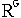
\includegraphics{misc/academicons_rgate} & \href{https://www.researchgate.net/profile/Kevin_Godin-Dubois2}{ResearchGate} \\     
  \end{tabular}
 }
 \\\\
 
 \itm{Synopsis}{}{
  {\centering\large \emph{A-Life Researcher on the Emergence of Cognition}}%
  \\\small
  After a PhD thesis focused on artificial plant-like lifeforms and their dynamics at the evolutionary scale, I plan on returning to my core interest: artificial cognition.
  More specifically, my objectives are to investigate the mechanisms by which high-level forms of interaction can be built upon low-level inputs/outputs, especially in response to environmental constraints.
 }%
 \\
 
 \itm{Interests}{}{%
 \hfill
 \foreach \i/\l in {mew/Morphogenetic Engineering\cite{Dubois2017},
                    phylogenetics_colored/{Species Dynamics}\cite{GodinDubois2019b,GodinDubois2019c},
                    splinoids_combat/Artificial Cognition\cite{GodinDubois2020b}} {
  \begin{minipage}[t]{.2\textwidth}
   \centering
   \includegraphics[width=\textwidth]{annexes/\i} \\
   \l
  \end{minipage}
  \hfill
 } 
 }
\end{sect}

\begin{sect}{Education}
 \itm{PhD}{2016 - July 2020}{%
  Toulouse University, France \\
  Thesis title: \emph{``Environment-driven speciation: long term interactions in artificial plant communities''} \\
  {\small Investigated how complexification of artificial creatures could be further enhanced by moving the control apparatus around the abiotic component of an ecosystem } \\
  \textbf{Contact:} Pr. Y. Duthen (\mailto{Yves.Duthen@irit.fr})
 }
 \\
   
 \itm{Master}{2014 - 2016}{
  Toulouse University, France \\
  {\small Artificial intelligence: mathematical \& symbolic models, training methods}
 }
 \\
 
 \itm{Bachelor}{2011 - 2014}{
  Toulouse University, France \\
  {\small Computer science: Networks, Programming, Systems, Mathematics}
 }
\end{sect}

% \newpage
\begin{sect}{Experience}
 \itm{Teachings}{2017 - 2019}{
  Capitole University, Toulouse, France \\
  \di L2 Excel and Visual Basic for Applications \\
  \di L2 Algorithms and Visual Basic \\
  \di L3 Modeling in Database \\
 }
 \\
 
 \itm{Teachings}{2016 - 2017}{%
  Paul Sabatier University, Toulouse, France \\
  \di L2 project monitoring on C programming \\
 }
 \\
 
 \itm{Internship}{2016 (6 months)}{%
  Toulouse Research Institute on Computer Science (IRIT), France \\%
  \emph{``Rule-based artificial embryogenesis in a complex 3D environment''} \\%
  {\small Deployed rule-based genomes on the MecaCell platform to study artificial plant growth and cell specialization.}%
 }
 \\
 
 \itm{Internship}{2015 (3 months)}{
  \emph{``Comparison of different evolutionary approaches, an application to the GECCO 2015 challenge''} \\
  {\small Performed a performance comparison (accuracy, efficiency) between Artificial Neural and Genetic Regulatory Networks on the 2015 GECCO temperature prediction challenge data.} \\
  \textbf{Contact:} Pr. H. Luga (\mailto{Herve.Luga@irit.fr})
 }
 \\
 
 \itm{Internship}{2014 (2 months)}{
  \emph{``Conception of an architecture for automated bird discrimination''} \\
  {\small Applied Hidden Markov Models to the BirdClef2014 challenge on the identification of specific bird species in a corpus of thousands of recordings.} \\
  \textbf{Contact:} Pr. J. Farnias (\mailto{Jerome.Farinas@irit.fr})
 }
\end{sect}

\newcommand{\formatskill}[2]{\skilldisk{#2} \small#1}
\def\cols(#1)#2{%
 \itm{#1}{}{%
  \foreach \p/\l in {#2} {%
   \begin{minipage}{.32\rwidth}\formatskill{\l}{\p}\end{minipage}%
  }%
 }%
}
\begin{sect}{Skills}
 \cols(Programming){%
  90/C++,
  80/{C, Java},
  70/Python}%
  
 \cols(Processing){%
  90/{Bash (sed, awk ...)},
  85/Gnuplot,
  70/{Octave/Matlab}
 }
 
 \cols(Redaction){%
  85/{\LaTeX /Ti\textit{k}Z},
  75/Office Software
 }
 
 \cols(Systems){%
  85/Linux,
  70/{Windows, Android}
 }

 \cols(Languages){%
  95/French,
  90/English
 }
\end{sect}
 
\begin{sect}{Scholarships and Fellowships}
 \itm{2016}{70K \euro}
     {PhD Fellowship from the French Minister of Higher Education and Research (MESR) - over 3 years}
 \\
 
 \itm{2015}{10K \euro}
     {Master Scholarship from the International Mathematics and Computer Science Center (LabEx CIMI, Toulouse)}
 \\
     
 \itm{2014}{3K6 \euro}
     {Merit Scholarship from the Regional Student Welfare Office (CROUS, Toulouse) - over 2 years}
\end{sect}

\newpage
\begin{sect}[]{Research Output}
 \multicolumn{1}{m{\lwidth}}{} & \multicolumn{1}{m{\rwidth-11.6pt}}{} \\*
\end{sect}%
\vspace{-\baselineskip}
\nocite{*}%
\textbf{Pending publication}
\printbibliography[heading=none, type=unpublished]
\textbf{Peer-reviewed publications}
\printbibliography[heading=none, nottype=misc,nottype=unpublished]
\textbf{Oral presentations}
\printbibliography[heading=none, nottype=unpublished, subtype=talk]

\end{document}
